\documentclass[12pt]{scrartcl}
\usepackage{amsmath,amssymb,amsfonts,mathrsfs}
\usepackage{miller}
\usepackage{multirow}
\usepackage{subeqnarray}
\usepackage{bm}
\usepackage{natbib}

\usepackage{graphicx}
\graphicspath{{./}{./figure/}{../Figures/}}
\DeclareGraphicsExtensions{.pdf,.png}
\usepackage[pdftex,                                     % hyper-references for pdftex
bookmarksnumbered=true,%                                % generate bookmarks with numbers
%pagebackref=true,%                                      % generate backref in biblio
colorlinks=true,%
linkcolor=blue,
citecolor=red,
urlcolor=blue,
pdfpagelabels=false,
plainpages = false,
]{hyperref}%

\usepackage[capitalise]{cleveref}                                   % for clever referencing


\usepackage{tikz}
\usetikzlibrary{shapes.geometric, arrows}
\usetikzlibrary{automata,positioning}


% SOMETHING USEFUL
\newcommand{\ie}{\textit{i.e.}}
\newcommand{\eg}{\textit{e.g.}}
\newcommand{\cf}{\textit{cf.}}
\newcommand{\Euler}{\term{Euler}}
\newcommand{\Gauss}{\term{Gauss}}
\newcommand{\Fourier}{\term{Fourier}}

\newcommand{\kB}{\ensuremath{k_\text{B}}}

% FUNCTIONS AND OPERATORS
\newcommand{\transpose}[1]{\ensuremath{{#1}^{\text T}}}
\newcommand{\inverse}[1]{\ensuremath{{#1}^{-1}}}
\newcommand{\invtranspose}[1]{\ensuremath{{#1}^{\text{-T}}}}
\newcommand{\sign}[1]{\ensuremath{\operatorname{sgn}\left({#1}\right)}}
\newcommand{\grad}[1][]{\ensuremath{\operatorname{grad}{#1}}}
\newcommand{\Grad}[1][]{\ensuremath{\operatorname{Grad}{#1}}}
\newcommand{\divergence}[1][]{\ensuremath{\operatorname{div}{#1}}}
\newcommand{\Divergence}[1][]{\ensuremath{\operatorname{Div}{#1}}}
\newcommand{\curl}[1][]{\ensuremath{\operatorname{curl}{#1}}}
\newcommand{\Curl}[1][]{\ensuremath{\operatorname{Curl}{#1}}}
\newcommand{\totalder}[2]{\ensuremath{\frac{\inc{#1}}{\inc{#2}}}}
\newcommand{\partialder}[2]{\ensuremath{\frac{\partial{#1}}{\partial{#2}}}}
\newcommand{\inc}[1]{\ensuremath{\text d{#1}}}
\newcommand{\abs}[1]{\ensuremath{\left|{#1}\right|}}
\newcommand{\norm}[2][]{\ensuremath{\left|\left|{#2}\right|\right|\if\relax\detokenize{#1}\relax\else _{#1}\fi}}
\newcommand{\avg}[1]{\ensuremath{\overline{#1}}}
\newcommand{\fluct}[1]{\ensuremath{\widetilde{#1}}}
\newcommand{\FT}[1]{\ensuremath{\mathcal F\left[{#1}\right]}}
\newcommand{\invFT}[1]{\ensuremath{\mathcal F^{-1}\left[{#1}\right]}}

\newcommand{\domain}[1]{\ensuremath{\mathcal{#1}}}
\newcommand{\tnsrfour}[1]{\ensuremath{\mathbb{#1}}}
\newcommand{\tnsr}[1]{\ensuremath{\mathbf{#1}}}
\newcommand{\tnsrgreek}[1]{\ensuremath{\bm{#1}}}
\newcommand{\vctr}[1]{\ensuremath{\mathbf{#1}}}
\newcommand{\vctrgreek}[1]{\ensuremath{\bm{#1}}}

% SPECIAL TENSORS
\newcommand{\eyetwo}{\ensuremath{\tnsr I}}
\newcommand{\eyefour}{\ensuremath{\tnsrfour I}}

% VARIABLES
\newcommand{\defmap}{\ensuremath{\vctrgreek{\chi}}}
\newcommand{\stiffness}{\tnsrfour C}
\newcommand{\fPK}{\ensuremath{\tnsr P}}
\newcommand{\fPKcomponent}{\ensuremath{P}}
\newcommand{\fPKavg}{\ensuremath{\avg{\fPK}}}
\newcommand{\sPK}{\ensuremath{\tnsr S}}
\newcommand{\F}[1][]{\ensuremath{\tnsr F^{#1}}}
\newcommand{\Fcomponent}[1][]{\ensuremath{F^{#1}}}
\newcommand{\Fdot}[1][]{\ensuremath{\dot{\tnsr F}^{#1}}}
\newcommand{\E}{\tnsr E}
\newcommand{\GL}{\ensuremath{\tnsr E_\text{e}}}
\newcommand{\Favg}{\ensuremath{\avg{\F}}}
\newcommand{\Ffluct}{\ensuremath{\fluct{\F}}}
\newcommand{\Fp}[1][]{\ensuremath{\tnsr F_\text{p}^{#1}}}
\newcommand{\Fpdot}[1][]{\ensuremath{\dot{\tnsr F}_\text{p}^{#1}}}
\newcommand{\Fe}[1][]{\ensuremath{\tnsr F_\text{e}^{#1}}}
\newcommand{\velgrad}{\ensuremath{\tnsr L}}
\newcommand{\Lp}{\ensuremath{\tnsr L_\text{p}}}
\newcommand{\bcFdot}{\ensuremath{\dot{\tnsr F}_\text{BC}}}
\newcommand{\bcF}{\ensuremath{{\F}_\text{BC}}}
\newcommand{\bcfPK}{\ensuremath{{\fPK}_\text{BC}}}
\newcommand{\Burgers}[1]{\ensuremath{\vctr b^{#1}}}
\newcommand{\n}[1]{\ensuremath{\vctr n^{#1}}}
\newcommand{\velocity}[2]{\ensuremath{v^{#1}_\text{#2}}}
\newcommand{\galpha}{\ensuremath{\gamma^{\alpha}}}
\newcommand{\dotgalpha}{\ensuremath{\dot{\gamma}^{\alpha}}}
\newcommand{\cs}{\ensuremath{\tnsrgreek \sigma}}

\newif\ifcuboidshade
\newif\ifcuboidemphedge

\tikzset{
  cuboid/.is family,
  cuboid,
  shiftx/.initial=0,
  shifty/.initial=0,
  dimx/.initial=3,
  dimy/.initial=3,
  dimz/.initial=3,
  scale/.initial=1,
  densityx/.initial=1,
  densityy/.initial=1,
  densityz/.initial=1,
  rotation/.initial=0,
  anglex/.initial=0,
  angley/.initial=90,
  anglez/.initial=225,
  scalex/.initial=1,
  scaley/.initial=1,
  scalez/.initial=0.5,
  front/.style={draw=black,fill=white},
  top/.style={draw=black,fill=white},
  right/.style={draw=black,fill=white},
  shade/.is if=cuboidshade,
  shadecolordark/.initial=black,
  shadecolorlight/.initial=white,
  shadeopacity/.initial=0.15,
  shadesamples/.initial=16,
  emphedge/.is if=cuboidemphedge,
  emphstyle/.style={thick},
}


% TIKZ extension
\newcommand{\tikzcuboidkey}[1]{\pgfkeysvalueof{/tikz/cuboid/#1}}

% Commands
\newcommand{\tikzcuboid}[1]{
    \tikzset{cuboid,#1} % Process Keys passed to command
  \pgfmathsetlengthmacro{\vectorxx}{\tikzcuboidkey{scalex}*cos(\tikzcuboidkey{anglex})*28.452756}
  \pgfmathsetlengthmacro{\vectorxy}{\tikzcuboidkey{scalex}*sin(\tikzcuboidkey{anglex})*28.452756}
  \pgfmathsetlengthmacro{\vectoryx}{\tikzcuboidkey{scaley}*cos(\tikzcuboidkey{angley})*28.452756}
  \pgfmathsetlengthmacro{\vectoryy}{\tikzcuboidkey{scaley}*sin(\tikzcuboidkey{angley})*28.452756}
  \pgfmathsetlengthmacro{\vectorzx}{\tikzcuboidkey{scalez}*cos(\tikzcuboidkey{anglez})*28.452756}
  \pgfmathsetlengthmacro{\vectorzy}{\tikzcuboidkey{scalez}*sin(\tikzcuboidkey{anglez})*28.452756}
  \begin{scope}[xshift=\tikzcuboidkey{shiftx}, yshift=\tikzcuboidkey{shifty}, scale=\tikzcuboidkey{scale}, rotate=\tikzcuboidkey{rotation}, x={(\vectorxx,\vectorxy)}, y={(\vectoryx,\vectoryy)}, z={(\vectorzx,\vectorzy)}]
    \pgfmathsetmacro{\steppingx}{1/\tikzcuboidkey{densityx}}
  \pgfmathsetmacro{\steppingy}{1/\tikzcuboidkey{densityy}}
  \pgfmathsetmacro{\steppingz}{1/\tikzcuboidkey{densityz}}
  \newcommand{\dimx}{\tikzcuboidkey{dimx}}
  \newcommand{\dimy}{\tikzcuboidkey{dimy}}
  \newcommand{\dimz}{\tikzcuboidkey{dimz}}
  \pgfmathsetmacro{\secondx}{2*\steppingx}
  \pgfmathsetmacro{\secondy}{2*\steppingy}
  \pgfmathsetmacro{\secondz}{2*\steppingz}
  \foreach \x in {\steppingx,\secondx,...,\dimx}
  { \foreach \y in {\steppingy,\secondy,...,\dimy}
    {   \pgfmathsetmacro{\lowx}{(\x-\steppingx)}
      \pgfmathsetmacro{\lowy}{(\y-\steppingy)}
      \filldraw[cuboid/front] (\lowx,\lowy,\dimz) -- (\lowx,\y,\dimz) -- (\x,\y,\dimz) -- (\x,\lowy,\dimz) -- cycle;
    }
    }
  \foreach \x in {\steppingx,\secondx,...,\dimx}
  { \foreach \z in {\steppingz,\secondz,...,\dimz}
    {   \pgfmathsetmacro{\lowx}{(\x-\steppingx)}
      \pgfmathsetmacro{\lowz}{(\z-\steppingz)}
      \filldraw[cuboid/top] (\lowx,\dimy,\lowz) -- (\lowx,\dimy,\z) -- (\x,\dimy,\z) -- (\x,\dimy,\lowz) -- cycle;
        }
    }
    \foreach \y in {\steppingy,\secondy,...,\dimy}
  { \foreach \z in {\steppingz,\secondz,...,\dimz}
    {   \pgfmathsetmacro{\lowy}{(\y-\steppingy)}
      \pgfmathsetmacro{\lowz}{(\z-\steppingz)}
      \filldraw[cuboid/right] (\dimx,\lowy,\lowz) -- (\dimx,\lowy,\z) -- (\dimx,\y,\z) -- (\dimx,\y,\lowz) -- cycle;
    }
  }
  \ifcuboidemphedge
    \draw[cuboid/emphstyle] (0,\dimy,0) -- (\dimx,\dimy,0) -- (\dimx,\dimy,\dimz) -- (0,\dimy,\dimz) -- cycle;%
    \draw[cuboid/emphstyle] (0,\dimy,\dimz) -- (0,0,\dimz) -- (\dimx,0,\dimz) -- (\dimx,\dimy,\dimz);%
    \draw[cuboid/emphstyle] (\dimx,\dimy,0) -- (\dimx,0,0) -- (\dimx,0,\dimz);%
    \fi

    \ifcuboidshade
    \pgfmathsetmacro{\cstepx}{\dimx/\tikzcuboidkey{shadesamples}}
    \pgfmathsetmacro{\cstepy}{\dimy/\tikzcuboidkey{shadesamples}}
    \pgfmathsetmacro{\cstepz}{\dimz/\tikzcuboidkey{shadesamples}}
    \foreach \s in {1,...,\tikzcuboidkey{shadesamples}}
    {   \pgfmathsetmacro{\lows}{\s-1}
        \pgfmathsetmacro{\cpercent}{(\lows)/(\tikzcuboidkey{shadesamples}-1)*100}
        \fill[opacity=\tikzcuboidkey{shadeopacity},color=\tikzcuboidkey{shadecolorlight}!\cpercent!\tikzcuboidkey{shadecolordark}] (0,\s*\cstepy,\dimz) -- (\s*\cstepx,\s*\cstepy,\dimz) -- (\s*\cstepx,0,\dimz) -- (\lows*\cstepx,0,\dimz) -- (\lows*\cstepx,\lows*\cstepy,\dimz) -- (0,\lows*\cstepy,\dimz) -- cycle;
        \fill[opacity=\tikzcuboidkey{shadeopacity},color=\tikzcuboidkey{shadecolorlight}!\cpercent!\tikzcuboidkey{shadecolordark}] (0,\dimy,\s*\cstepz) -- (\s*\cstepx,\dimy,\s*\cstepz) -- (\s*\cstepx,\dimy,0) -- (\lows*\cstepx,\dimy,0) -- (\lows*\cstepx,\dimy,\lows*\cstepz) -- (0,\dimy,\lows*\cstepz) -- cycle;
        \fill[opacity=\tikzcuboidkey{shadeopacity},color=\tikzcuboidkey{shadecolorlight}!\cpercent!\tikzcuboidkey{shadecolordark}] (\dimx,0,\s*\cstepz) -- (\dimx,\s*\cstepy,\s*\cstepz) -- (\dimx,\s*\cstepy,0) -- (\dimx,\lows*\cstepy,0) -- (\dimx,\lows*\cstepy,\lows*\cstepz) -- (\dimx,0,\lows*\cstepz) -- cycle;
    }
    \fi 

  \end{scope}
}

\begin{document}

\title{CyXtal: C(P)ython Package for Crystal Plasticity Data Analysis}
\subtitle{development note}
\author{Chen Zhang}
\maketitle

\section{Module: ctools}

\section{Module: cxtallite}

\section{External Module: ext\_aps}

\subsection{parsers.py}
This particular module include several function that help facilitate the analysis of data collected at beamline-34-ID-E at Advanced Photon Source in Argonne National Lab.
%
\begin{enumerate}

\item \textbf{parser\_xml(\ldots)} \\

\item \textbf{strain\_refine(\ldots)} \\
The DAXM characterization uses white beam to capture a convoluted diffraction patterns from the entire volume.
Then a Pt wire, also known as the differential aperture, is used to block the diffraction signals from certain voxels.
During the post processing, deconvolution of the diffraction patterns is performed to extract the Laue diffraction pattern for each voxel, thus to achieve spatially revolved characterization of the material.

Since the final results are essentially Laue diffraction patterns, all the analysis that can be used for Laue diffraction can be applied to the DAXM data as well.
Particularly, it is possible to extract the crystal rotation and lattice strain by analyzing the mismatch between ideal diffraction spots (zero rotation, strain free) and measured diffraction spots.
The underlying assumption is that the deformation of the crystal can be resolved into two steps: a simple rotation that causes diffraction peaks to shift and a small lattice stretch that causes diffraction peaks to deviate slightly from its ideal location (\cref{fig:srefine}).

\begin{figure}[htp]
\centering
%!TEX root = development.tex

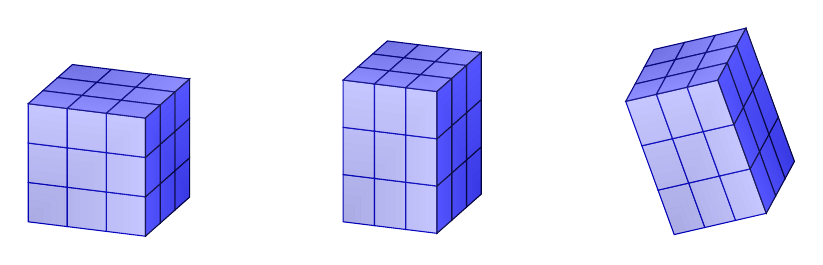
\begin{tikzpicture}

     \tikzcuboid{%
    shiftx=0cm,%
    shifty=0cm,%
    scale=0.50,%
    rotation=0,%
    densityx=1,%
    densityy=1,%
    densityz=1,%
    front/.style={draw=blue!75!black,fill=blue!25!white},%
    right/.style={draw=blue!25!black,fill=blue!75!white},%
    top/.style={draw=blue!50!black,fill=blue!50!white},%
    anglex=-7,%
    angley=90,%
    anglez=221.5,%
    scalex=1,%
    scaley=1,%
    scalez=0.5,%
    emphedge=false,%
    shade,%
    shadeopacity=0.1,%
    }
    
    \tikzcuboid{%
    shiftx=4cm,%
    shifty=0cm,%
    rotation=0,%
    shadeopacity=0.1,%
    scalex=0.8,%
    scaley=1.2,%
    scalez=0.5,%
    }
    
    \tikzcuboid{%
    shiftx=8cm,%
    shifty=0cm,%
    rotation=20,%
    shadeopacity=0.1,%
    scalex=0.8,%
    scaley=1.2,%
    scalez=0.5,%
    }
\end{tikzpicture}
\caption{%
According to continue mechanics theory, the plastic deformation can be resolved into stretching (\tnsr U) and rotation (\tnsr R) and , namely $\tnsr F = \tnsr R \tnsr U$. }
\label{fig:srefine}
\end{figure}

Assuming small lattice strain present in the sample, the indexation program executed at APS uses forward prediction method to match the diffraction spots while ignoring the streaking effect present in the diffraction patterns.
The results of this indexation is a set of reciprocal lattice vectors with no strain present (strain free).
In other words, the diffraction spots calculated from these set of reciprocal lattice vectors will differ from those measured.
This mismatch between calculation and measurements can be attributed to experimental error and residual lattice.
Since the indexation results (*.xml file) also contains the measured diffraction vectors used to identify the reciprocal lattice vectors, it is possible to further process the data to extract the lattice strain.
The strain refinement algorithm used in this package is based on the software package ``LaueGo'' developed and maintained by Dr.Tischler at APS, ANL.
\footnote{\url{http://www.aps.anl.gov/Sectors/33_34/microdiff/}}

Assuming that the residual mismatch between the theoretical diffraction peaks and measured diffraction peaks are the results of residual lattice strain, it is possible to construct a strained unit cell that generate a diffraction pattern that fits the measurement better.
Comparing the strained unit cell and the ideal unit cell, a deformation gradient (\tnsr F) can be calculated by
\[
	\tnsr B_\text{strained} = \tnsr F \: \tnsr B_\text{ideal}
\]
where \tnsr B is the basis tensor whose column vectors are unit cell base vectors.

With \tnsr F known, the Green strain tensor can be calculate by
\begin{align*}
	\tnsr C &= \tnsr F^T \tnsr F \\
	            &= (1 + \tnsr \epsilon)^2 \\
	            &= 1 + 2\epsilon + \epsilon^2 \\
	            &\approx 1 + 2\epsilon + O(\epsilon^2)
\end{align*}

So the lattice strain for given voxel can be approximated by
\[
	\epsilon = \dfrac{1}{2} (\tnsr F^T\tnsr F - \tnsr I)
\]

% algorithm used in the code
Since there is no explicit method available to find a strained unit cell that generates better diffraction pattern, it is inevitable to use an implicit numeric approach to locate a possible solution.
The overall goal of this implicit numeric approach is to minimize the difference between the calculated diffraction peaks and the measured ones.
To quantify the mismatch, angular difference between all diffraction peak pairs (calculated and measured),
\[
	err = 1 - \dfrac{1}{N} \sum \tnsr q_\text{calculated} \cdot \tnsr q_\text{measured}
\]
where $\tnsr q_\text{calculated}$ can be calculated by
\[
	\tnsr q_\text{calculated} = \tnsr B^*_\text{strained} \cdot \vctr v_\text{hkl}.
\]

Here $\tnsr B^*_\text{strained}$ is the basis in reciprocal space whose columnar vectors are the reciprocal base vectors and $\vctr v_\text{hkl}$ is the indexation for the diffraction peak.
The relationship between $\tnsr B$ and $\tnsr B^*$ can be found through
\[
	\tnsr B^* = 2 \pi \tnsr B^{-T}
\]

One of the problem of using numerical approach is that it might leads to a set of lattice constants that satisfy our criterion but completely unrealistic. 
To avoid situation like this, the objective function for the optimization of strain refinement is constructed with both the mismatch of \tnsr Q as well as the change in the volume of the unit cell, 
\[
	F(\tnsr x) = 1 - \dfrac{1}{N} \sum \tnsr q_\text{calculated} \cdot \tnsr q_\text{measured}
\]
where \tnsr x represents the lattice constant vector, $\tnsr x = (a,b,c,\alpha,\beta,\gamma)$

Considering most of the searching will be done in the reciprocal space, it is necessary to find the connection between $\tnsr B^*$ and \tnsr F.

Let $\tnsr B_2$ be the basis for strained and rotated unit cell, $\tnsr B_0$ be the basis for ideal unit cell (zero rotation, strain free), and $\tnsr B_1$ be the basis for the unit cell only considering stretch.
\[
	\tnsr B_2 = \tnsr F \tnsr B_0 = \tnsr R \tnsr B_1 = \tnsr R \tnsr U \tnsr B_0
\]
where \tnsr R represents the lattice rotation and \tnsr U represents the lattice stretch.

Convert everything to reciprocal space except for \tnsr F,
\footnote{Inverse transpose does not change the order of matrix multiplication.}
\begin{align*}
	\tnsr B_2 &= \tnsr F \tnsr B_0 \\
	\tnsr B^*_2 &= \tnsr F^{-T} \tnsr B_0^*
\end{align*}
Now the deformation gradient can be expressed using reciprocal basis,
\[
	\tnsr F = {\tnsr B_2^*}^{-T} {\tnsr B_0^*}^T
\]
Thus the strain tensor can be written as
\begin{align*}
	\epsilon &= \dfrac{1}{2} (\tnsr F^T\tnsr F - \tnsr I) \\
	              &= \dfrac{1}{2} ( ({\tnsr B_2^*}^{-T} {\tnsr B_0^*}^T)^T{\tnsr B_2^*}^{-T} {\tnsr B_0^*}^T - \tnsr I) \\
	              &= \dfrac{1}{2} ( \tnsr B_0^* {\tnsr B_2^*}^{-1} {\tnsr B_2^*}^{-T} {\tnsr B_0^*}^T  - \tnsr I)
\end{align*}

Considering that rotation is not reflected in the Green strain tensor,
\[
	\tnsr F^T \tnsr F = \tnsr U^T \tnsr R^T \tnsr R \tnsr U = \tnsr U^T \tnsr U
\]
it is possible to skip the last rotation by using $\tnsr U =  {\tnsr B_1^*}^{-T} {\tnsr B_0^*}^T$
\begin{align*}
	\epsilon &=  \dfrac{1}{2} (\tnsr U^T\tnsr U - \tnsr I) \\
	              &=  \dfrac{1}{2} ( \tnsr B_0^* {\tnsr B_1^*}^{-1} {\tnsr B_1^*}^{-T} {\tnsr B_0^*}^T  - \tnsr I)
\end{align*}
Since all reciprocal lattice vectors are in APS coordinate system(\cref{sec:coord}), the strain tensor calculated here is also in the APS coordinate system.
\footnote{If the strain is really small, the lattice strain tensor can be further simplified to $\epsilon = \tnsr U - \tnsr  I$.} 

Another point worth mentioning here is that the full strain tensor can only be ``guessed'' when the beam energy is known.
In other words, without the knowledge of the length of \tnsr q (diffraction vector), it is not possible to inferred the whole strain tensor.
However, if the volume of the unit cell is assumed to remain constant through deformation, the deviatoric component of the strain tensor is not tied to $||\tnsr q||$.
\footnote{Diffraction vector: $\tnsr q_{hkl} = \tnsr B \cdot (khl) $}
Thus, it is necessary to add this assumption to the optimization if white beam calibration is not done.

Originally the deviatoric strain is directly extracted using 
\[
	\tnsr \epsilon_{dev} = \tnsr \epsilon - \dfrac{1}{3}\text{tr}(\tnsr \epsilon),
\]
which results in large residual strain value. 
To avoid this problem, it is recommended to remove the deviatoric at the deformation gradient level, $\tnsr F$.
\footnote{%
Dr. Eisenlohr found some reference on computing the deviatoric strain directly from deformation gradient rather than the strain tensor.
}
The overall deformation gradient can be decomposed into volumetric change (hydrostatic, $\tnsr F_v$) and the deviatoric change (deviatoric, $\tnsr F_D$),
\[ 
	\tnsr F = \tnsr F_v \tnsr F_D
\]

The volumetric change, $\tnsr F_v$ is defined as 
\[
	\tnsr F_v = J^{\frac{1}{3}} \tnsr I
\]
where $J = \det (F)$.
Thus the deviatoric portion of the deformation gradient can be expressed as 
\[
	\tnsr F_D = J^{-\frac{1}{3}} \tnsr F
\]
The deviatoric strain now can be expressed as 
\[
	\tnsr \epsilon_D = \tnsr \epsilon - \tnsr \epsilon_v
\]
in which 
\[
	\tnsr \epsilon = \dfrac{1}{2} (\tnsr U^T\tnsr U - \tnsr I), 
	\tnsr \epsilon_v = \dfrac{1}{2} (J^{\frac{2}{3}} - 1)\tnsr I
\]
Thus,
\[
	\tnsr \epsilon_D = \dfrac{1}{2} ( \tnsr U_D^2- \tnsr I) J^{\frac{2}{3}}
\]
where $\tnsr U_D^2 = \tnsr F_D^T \tnsr F_D$.

Define the correction term as $\delta$ to connect deviatoric strain with full strain tensor, we have
\[
	\tnsr \epsilon_D = \tnsr \epsilon - \tnsr \epsilon_v 
	                          = \dfrac{1}{2} (\tnsr U^T\tnsr U - \tnsr I) + \delta
\]
where $\delta = -\epsilon_v = \dfrac{1}{2} (1 - J^{\frac{2}{3}})\tnsr I$
\footnote{%
$\delta$ is essentially the correction factor that correct the error from volume change during optimization procedure.
}

\end{enumerate}


\section{External Module: ext\_damask}

\section{External Module: ext\_vtk}

\section{Appendix}
\subsection{Find Base Vectors from Lattice Constants}
\label{sec:lc2bv}
In the strain refinement, one important step is to find the reciprocal lattice vectors from given lattice constants.
The easiest way to find the reciprocal lattice vectors is to find its dual, real space lattice vectors.

\begin{figure}[htp]
\centering
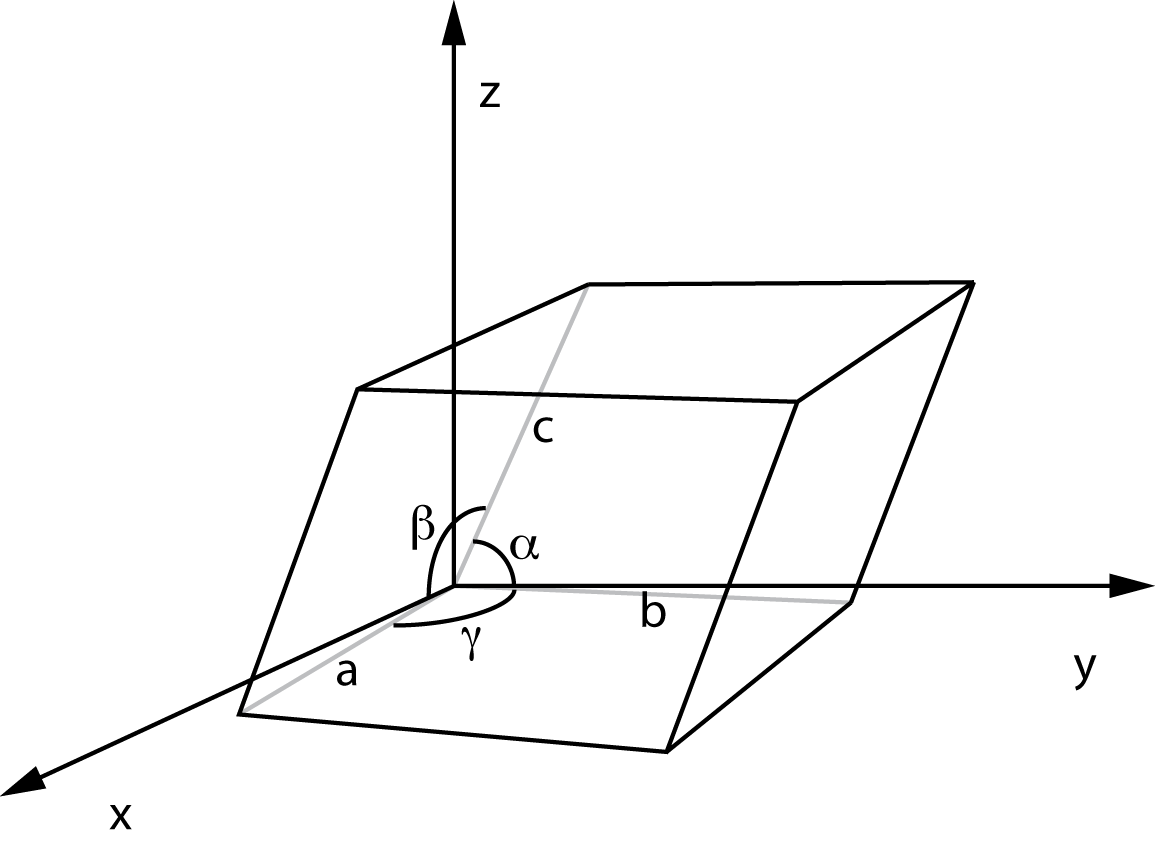
\includegraphics[width=.7\linewidth]{UnitCell.png}
\caption{A general unit cell with its six lattice constants}
\label{fig:unitcell}
\end{figure}

\cref{fig:unitcell} shows an example of unit cell randomly oriented in space.
Although there are six parameters ($a,b,c, \alpha, \beta, \gamma$) available to describe the shape of the unit cell, the exact numerical representation of the unit cell, namely the base lattice vectors, is not easy to determine.

To make the math a little bit easier, let assume that \vctr a is align with x-axis, which gives us
\[
	\vctr a = (a_1, a_2, a_3) = (a, 0, 0)
\]
Then let's determine the x-y plane through \vctr a and \vctr b.
In other words, \vctr b can be easily written out as
\[
	\vctr b = (b_1, b_2, b_3) = (b\cos\gamma, b\sin\gamma, 0)
\]
For a general unit cell, the volume of the cell is determined through its six lattice parameters/constants,
\[
	V = abc\sqrt{1 + 2\cos\alpha\cos\beta\cos\gamma - \cos^2\alpha-\cos^2\beta-\cos^2\gamma}
\]
The volume of the unit cell can also be calculated through
\[
	V = A_{xy}\cdot c_z = abc_3\sin\gamma
\]
which gives us
\[
	c_3 = \dfrac{V}{ab\sin\gamma}
\]
Arbitrary choice of the reference system should not affect the angle between two vectors, which gives us

\begin{align*}
	\vctr a \cdot \vctr c &= ac\cos\beta   = a_1c_1 + a_2c_2 + a_3c_3 \\
	\vctr b \cdot \vctr c &= bc\cos\alpha = b_1c_1 + b_2c_2 + b_3c_3
\end{align*}
Since \vctr a and \vctr b are known, we have
\begin{align*}
	a_1c_1 + 0 + 0 &= ac_1 = ac\cos\beta \\
	b_1c_1 + b_2c_2 + 0 &= bc_1\cos\gamma  + bc_2\sin\gamma  = bc\cos\alpha
\end{align*}
Solve the above linear system, we have
\begin{align*}
	c_1 &= c\cos\beta \\
	c_2 &= \dfrac{\cos\alpha - \cos\beta\cos\gamma}{\sin\gamma}c
\end{align*}
So the last base vector, \vctr c can be expressed as
\[
	\vctr c = ( c \: \cos\beta,
	                c \: \dfrac{\cos\alpha - \cos\beta\cos\gamma}{\sin\gamma},
	                \dfrac{V}{ab\sin\gamma})
\]
where $V$ is the volume of the unit cell.

To sum it up, for a general unit cell with six lattice parameters known, if we select \vctr a to be x-axis and \vctr b to lie in the x-y plane, the expression of base lattice vectors can be expressed as
\begin{align*}
	\vctr a &= (a, 0, 0) \\
	\vctr b &= (b\cos\gamma, b\sin\gamma, 0) \\
	\vctr c &= ( c \: \cos\beta,
	                c \: \dfrac{\cos\alpha - \cos\beta\cos\gamma}{\sin\gamma},
	                \dfrac{V}{ab\sin\gamma})
\end{align*}
where $V$ is the volume of the unit cell and can be calculate through
\[
	V = abc\sqrt{1 + 2\cos\alpha\cos\beta\cos\gamma - \cos^2\alpha-\cos^2\beta-\cos^2\gamma}.
\]

Another convection would be forcing \vctr b to be parallel to y-axis, however this convention has been dropped at APS.
Thus, there is no reason to consider this European convention anymore.

\subsection{Coordinates Transformation for DAXM Dataset}
\label{sec:coord}
Due to experiment setup of DAXM characterization, there are three different coordinate systems related to our data processing (\cref{fig:daxmcoord}):
\begin{itemize}
\item \textcolor{blue}{\textbf{XHF}} \\
This is the configuration closely tied to the sample.
During the scan, this configuration is used to control the sample stage for scanning. 
\footnote{The Beamline system has a internal conversion system converts the XHF to APS, which is then recorded in the XML output}

\item \textcolor{red}{\textbf{APS}} \\
This is the official coordinate system at APS, where the beam direction is the z-axis.
At beamline 34-ID-E, the indexation results is computed in this coordinate system.
In other words, the indexation results, including the reciprocal lattice and diffraction vectors (\tnsr q) are all in this coordinate system.
For some reason, the sample stage movement is also recorded in this coordinate system, which means all the data from the Beamline is in the APS configuration.

\item \textcolor{black}{\textbf{TSL}} \\
This coordinate system is closely tied to the sample where the sample surface normal is usually consider to be z-axis.
It is also the default coordinate system in TSL software, where OIM data is processed.
To make the coordinate system transformation easier, the x-axis in the TSL system is aligned with the x-axis in APS coordinate system.
However, this could be changed depending on how the sample is mounted in during EBSD and DAXM scan.

\end{itemize}

\begin{figure}[htp]
\centering
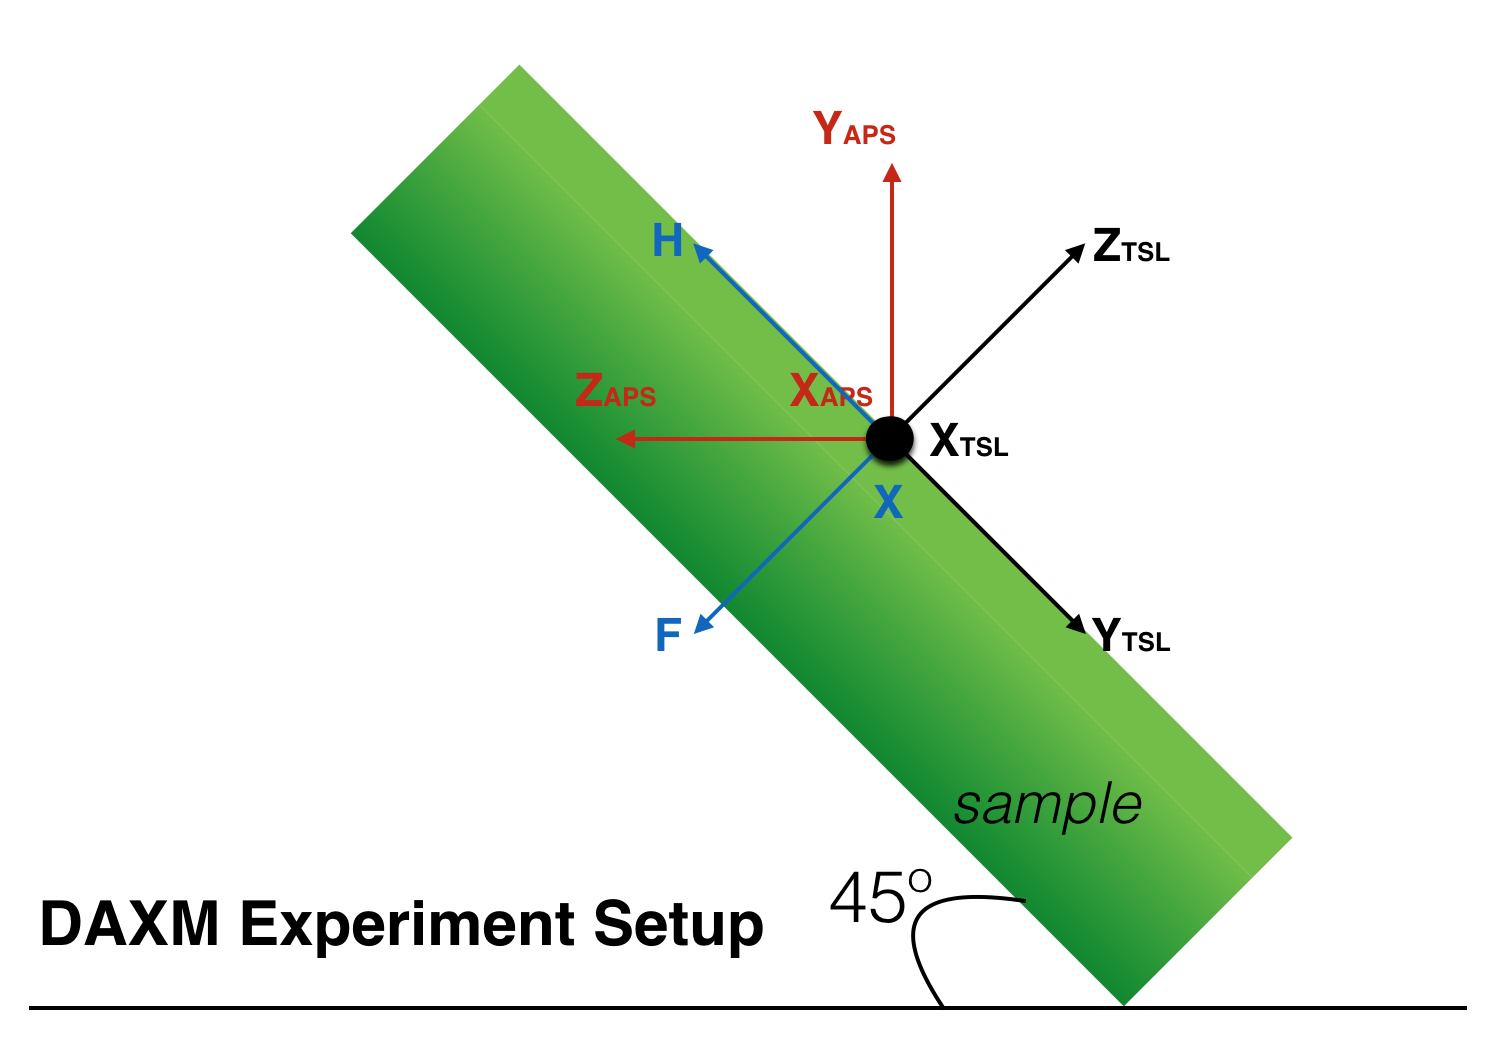
\includegraphics[width=.7\linewidth]{daxmcoord.png}
\caption{Three different coordinate system in DAXM characterization, assuming x-axis is shared by APS and TSL coordinate system.}
\label{fig:daxmcoord}
\end{figure}

\end{document}
